%File: formatting-instruction.tex
\documentclass[letterpaper]{article}
\usepackage{url,graphicx,xcolor}
\usepackage{times}
\usepackage{helvet}
\usepackage{courier}

\usepackage[hidelinks]{hyperref}
\usepackage[nameinlink]{cleveref}
\usepackage[
    % guidelines
]{faikrmod3}
\usepackage{booktabs}
\usepackage{multirow}
\usepackage{makecell}
\usepackage{array}
\usepackage{bookmark}
\usepackage{footnote}
\usepackage{lmodern}
\usepackage[numbers]{natbib}
\usepackage[bottom]{footmisc}
\frenchspacing
\usepackage[left=0.6in, right=0.6in, top=0.8in, bottom=0.85in]{geometry}

\hypersetup{pdfinfo={
Title={Title}
Author={Faezeh Sarlakifar}
}}
\setcounter{secnumdepth}{0}  
 \begin{document}
 	
% The file aaai.sty is the style file for AAAI Press 
% proceedings, working notes, and technical reports.
%
\title{A Probabilistic Approach to Diabetes Risk Assessment Using Bayesian Networks}
\author{Faezeh Sarlakifar\\
Master's Degree in Artificial Intelligence, University of Bologna\\
faezeh.sarlakifar@studio.unibo.it
}
\maketitle

\attention{DO NOT MODIFY THIS TEMPLATE - EXCEPT, OF COURSE FOR TITLE AND AUTHORS. REMOVE THE \texttt{guidelines} OPTION FROM  \texttt{$\backslash$usepackage[guidelines]\{faikrmod3\}} IN THE \LaTeX\ SOURCE IN THE FINAL VERSION.}

\begin{abstract}
\begin{quote}

Diabetes is a chronic and widespread health condition that affects many individuals worldwide. Early prediction and risk assessment are essential for effective prevention and management. In this study, the application of Bayesian Networks (BNs) to model the probabilistic relationships between health indicators and diabetes risk is explored. Multiple Bayesian structures are developed using Naïve Bayes, Hill Climbing (with various scoring methods), Simulated Annealing, and domain knowledge-driven techniques. To enhance model interpretability and predictive performance, a comprehensive feature selection approach is employed. The results demonstrate that Bayesian Networks offer an interpretable and robust framework for diabetes risk prediction, highlighting their potential for real-world healthcare applications.

\end{quote}
\end{abstract}


\section{Introduction}

\subsection{Domain}

In the field of medical health assessment, the interpretability and reliability of Artificial Intelligence (AI) methods are crucial, especially when it comes to conditions like diabetes. Healthcare professionals must be able to understand and trust the outcomes of predictive models to make informed decisions about patient care. Bayesian Networks (BNs) are particularly suitable for this purpose in diabetes risk assessment, as they provide a clear and interpretable framework that allows practitioners to understand the probabilistic relationships between various health indicators, such as age, BMI, and their impact on diabetes risk. This transparency is essential for building trust in AI models and ensuring they can be effectively integrated into clinical decision-making processes, ultimately improving patient outcomes.

This research is inspired by the study conducted by \citet{kong2024}, whose findings have been utilized to design the domain knowledge-based Bayesian Network model.

\subsection{Aim}

The goal of this project is to explore the effectiveness of Bayesian Networks (BNs) in modeling the probabilistic relationships between health indicators and diabetes risk. By leveraging different structure-learning approaches, the study aims to develop an effective and interpretable framework for diabetes risk assessment, evaluated using the area under the ROC curve (AUC-ROC) metric.

\subsection{Method} 

In this study, a Bayesian Network (BN) is built and evaluated using the ``\texttt{pgmpy}'' library. Several BN structures were explored, including Naïve Bayes, Hill Climbing (using various scoring functions: BIC, K2, and BDeu), Simulated Annealing, and a Domain Knowledge-based model.  

%To improve predictive performance and interpretability, a feature engineering step is applied to select the most important features for building the Bayesian Network. The SHAP (SHapley Additive exPlanations) values are defined to identify the most influential features. Implemented using the ``\texttt{SHAP}'' Python library. 

To improve predictive performance and interpretability, a feature engineering step is applied to select the most important features for building the Bayesian Network. SHAP (SHapley Additive exPlanations) values are employed to identify features importance, implemented using the ``\texttt{SHAP}'' Python library. These values are computed by training an XGBoost classifier \citep{XGBoost} and analyzing its explanations using TreeExplainer, a method specifically designed for tree-based models to capture complex nonlinear relationships. Since SHAP values provide a consistent measure of feature contribution in such models \citep{SHAP}, they serve as a robust criterion for feature selection. Based on these values, the top ten most influential features are selected for further modeling.

%\begin{enumerate}
%	\item SHAP (SHapley Additive exPlanations) values to identify the most influential features. Implemented using the ``\texttt{SHAP}'' Python library.
%	\item Mutual Information (MI) ranking, which measures statistical dependence between variables. Implemented using the ``\texttt{scikit-learn}'' Python library.
%\end{enumerate}

% Subsequently, the top 10 features are selected based on SHAP values.

% aligning with established diabetes risk factors from scientific literature and 

For parameter learning, the Conditional Probability Distributions (CPDs) are estimated using Maximum Likelihood Estimation (MLE) due to its efficiency in deterministic settings. The trained models are then evaluated using AUC-ROC scores to assess their classification performance.  

% Finally, the best-performing BN model is further analyzed to interpret probabilistic dependencies between diabetes risk factors.

\subsection{Results}

The experimental results show that, the Hill Climbing method (with K2 scoring), with an AUC score of 81.30, and the Domain Knowledge-driven method, with an AUC score of 83.57, effectively capture the relationships between features for diabetes risk assessment. These results suggest that both data-driven and expert-informed Bayesian Network structures can model the probabilistic relationships among health indicators.
% Furthermore, with increased computational resources for Bayesian structure learning and parameter learning, the models could potentially achieve higher predictive performance.

\section{Model}

In the proposed Bayesian Network, nodes represent key risk factors, while directed edges capture probabilistic dependencies based on expert knowledge and prior research. The variables—‘HighBP’, ‘GenHlth’, ‘HighChol’, ‘Age’, ‘Sex’, ‘Income’, ‘DiffWalk’, ‘BMI’, ‘HeartDiseaseorAttack’, and ‘Education’—were selected using SHAP values.

Figure 1 presents the Domain Knowledge Bayesian Network, illustrating the probabilistic dependencies between features.

%To ensure that the most relevant predictors were included, SHAP values were computed using an XGBoost classifier, a powerful gradient boosting model known for its ability to capture nonlinear interactions between features. SHAP values provide a consistent measure of feature contribution.

For structure learning, two complementary approaches were employed:
\begin{enumerate}
	\item Data-Driven Learning – Bayesian structures were learned using algorithms including Hill Climbing (BIC, K2, BDeu) and Simulated Annealing, optimizing for the highest AUC-ROC score. These models establish probabilistic relationships purely from data.
	\item Domain Knowledge-Based Network – A causally meaningful structure was designed based on established medical research, ensuring the relationships between variables align with known diabetes risk factors. The edges in this network reflect dependencies supported by scientific studies.
\end{enumerate}

\begin{figure}[ht]
	\centering
	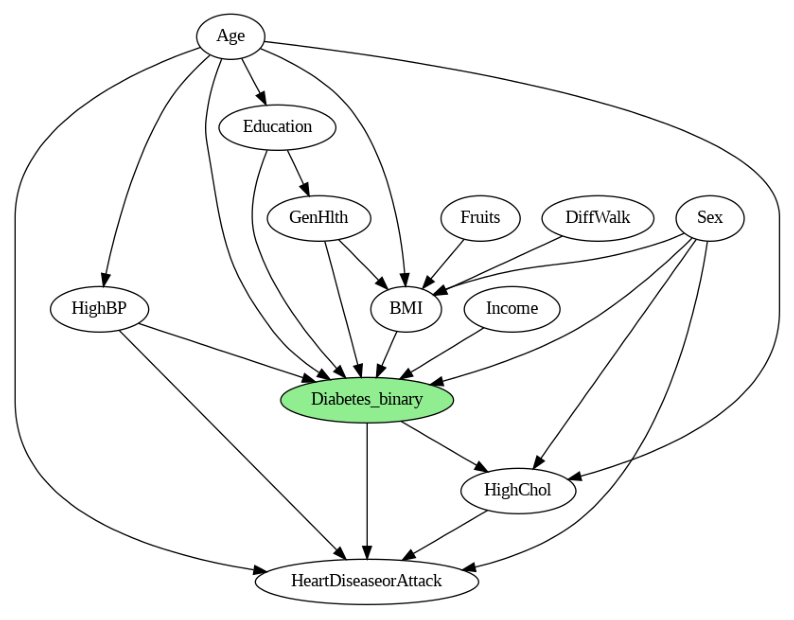
\includegraphics[width=0.5\textwidth]{images/bn-domain-knowledge.png}
	\caption{Proposed Bayesian Network.} 
	\label{fig:model}
\end{figure}

For parameter learning, Maximum Likelihood Estimation (MLE) was applied to estimate the Conditional Probability Distributions (CPDs).
%Among the trained models, the domain knowledge-based BN was selected for further analysis due to its strong performance and alignment with known risk factors.


\section{Analysis}

\subsection{Experimental setup}

This study employs the Diabetes Health Indicators dataset from the Behavioral Risk Factor Surveillance System (BRFSS). This dataset consists of 21 health-related features, which include demographics, lifestyle factors, and medical conditions. This makes the dataset a valuable resource for assessing diabetes risk. The dataset is then divided into training and validation sets. The training set is used to fit models, while the validation set serves to evaluate their performance. Models are compared using the AUC-ROC evaluation metric.


%This study employs the Diabetes Health Indicators dataset from the Behavioral Risk Factor Surveillance System (BRFSS). The cleaned dataset consists of 70,692 instances and 21 health-related features, which include demographics, lifestyle factors, and medical conditions. This makes the dataset a valuable resource for assessing diabetes risk. The dataset is then divided into training and validation sets. The training set is used to fit models, while the validation set serves to evaluate their performance. Models are compared using the AUC-ROC evaluation metric.

It was hypothesized that the domain knowledge-based model would outperform the others, as it is inspired by insights from scientific literature and incorporates relationships derived from the best-performing AI-based models. The results support this hypothesis, demonstrating the superiority of the domain knowledge-based approach. 

\subsection{Results}

Table 1 presents a comparison of the various methods experimented with for constructing the Bayesian Network. The results show that the Hill Climbing algorithm with the K2 scoring method outperforms other artificial intelligence-based models, and the domain knowledge-based approach surpasses all. Although the simulated annealing model was anticipated to perform better than Hill Climbing, the Hill Climbing with K2 scoring method proved to be more effective for diabetes risk assessment, which is an intriguing finding.
%\begin{table}[h]
%%	\centering
%	\caption{Comparison of AI-Based Bayesian Networks}
%	\begin{tabular}{lc}
%		\toprule
%		\textbf{Model} & \textbf{AUC Score} \\
%		\midrule
%		Hill Climbing (BIC)  & 76.80 \\
%		Hill Climbing (K2)   & 81.30 \\
%		Hill Climbing (BDeu) & 76.50 \\
%		Naïve Bayes          & 72.40 \\
%		Simulated Annealing  & 77.90 \\
%		\bottomrule
%	\end{tabular}
%	\label{tab:auc_comparison}
%\end{table}

%\begin{table}[h]
%	\centering
%	\caption{Comparison of AI-Based Bayesian Networks}
%	\resizebox{\linewidth}{!}{ % This makes the table fit within the subsection width
%		\begin{tabular}{l c}
%			\toprule
%			Bayesian Network Model & AUC Score \\
%			\midrule
%			Hill Climbing (BIC)        & 76.80 \\
%			Hill Climbing (K2)         & \textbf{81.30} \\
%			Hill Climbing (BDeu)       & 76.50 \\
%			Naïve Bayes                & 72.40 \\
%			Simulated Annealing        & 77.90 \\
%%			Domain Knowledge-Based Model & \textbf{TBD} \\
%			\bottomrule
%		\end{tabular}
%	}
%	\label{tab:bn_comparison}
%\end{table}

\begin{table}[h]
	\centering
	\caption{Comparison of Bayesian Network Models}
	\begin{tabular}{l@{\hspace{8 pt} }c}
		\toprule
		Bayesian Network Model & AUC Score \\
		\midrule
		Hill Climbing (BIC)        & 76.80 \\
		Hill Climbing (K2)         & 81.30 \\
		Hill Climbing (BDeu)       & 76.50 \\
		Naïve Bayes                & 72.40 \\
		Simulated Annealing        & 77.90 \\
		Proposed Model (domain knowledge-based) & \textbf{83.57} \\
		\bottomrule
	\end{tabular}
	\label{tab:bn_AI_based_comparison}
\end{table}


\section{Conclusion}
This study validates the effectiveness of Bayesian Networks for diabetes risk assessment, achieving an AUC-ROC score of 83.57 through the integration of domain knowledge from scientific literature. Furthermore, with increased computational resources for Bayesian structure learning and parameter learning, the models could potentially achieve higher predictive performance. The findings demonstrate that Bayesian Networks approach provides a valuable framework for diabetes risk prediction.

\section{Links to external resources}

\begin{itemize}
    \item The source code of this project is available at:  
    \\
    \href{https://github.com/faezesarlakifar/Unibo-FAIKR-M3-project}{\textcolor{blue}{GiHub repository}}
    \item You can find the utilized dataset at:
    \\ 
     \href{https://www.kaggle.com/datasets/alexteboul/diabetes-health-indicators-dataset}{\textcolor{blue}{Kaggle diabetes health indicators dataset}}
\end{itemize}

%\bigskip

%\bibliographystyle{aaai}
\bibliographystyle{plainnat}
\bibliography{faikrmod3.bib}

\attention{NOTICE: THIS REPORT'S LENGTH MUST NOT EXCEED \textbf{TWO PAGES} PLUS REFERENCES. THIS MAY MEAN THAT YOU WILL HAVE TO LEAVE OUT OF THE REPORT PART OF THE WORK YOU HAVE DONE OR OBSERVATIONS YOU HAVE. THIS IS NORMAL: THE REPORT SHOULD EMPHASIZE WHAT IS MOST SIGNIFICANT, NOTEWORTHY, AND REFER TO THE NOTEBOOK FOR ANYTHING ELSE. FOR ANY OTHER ASPECT OF YOUR WORK THAT YOU WOULD LIKE TO EMPHASIZE BUT CANNOT EXPLAIN HERE FOR LACK OF SPACE, FEEL FREE TO ADD COMMENTS IN THE NOTEBOOK.}





\end{document}